\chapter{Validation und Evaluation}
\label{cha:diskussion}

\section{Einführung und Abgrenzung}
\label{sec:eval_einfuehrung}

\todo{TODO}

\section{Validierung des Versuchsaufbaus}
\label{sec:eval_validierung}

TODO

\begin{table}[H]
    \centering
    \caption{Sanity-Kennzahlen der Hauptexperimente. Quelle: \texttt{ExperimentLogs.csv}.}
    \label{tab:eval_sanity}
    \begin{tabular}{lrrrrr}
        \hline
        Experiment & Klassen & Padding & Random-Basis & Failed (\%) & Pakete/Sample \\
        \hline
        exp-baseline-20      & 20  & OFF     & 5.0\,\%  & 1.7 & 635 \\
        exp-padding-20       & 20  & ON      & 5.0\,\%  & 1.5 & 638 \\
        exp-reduced-20       & 20  & Reduced & 5.0\,\%  & 1.9 & 611 \\
        exp-baseline-80      & 80  & OFF     & 1.2\,\%  & 4.4 & 583 \\
        exp-padding-80       & 80  & ON      & 1.2\,\%  & 4.5 & 601 \\
        exp-reduced-80       & 80  & Reduced & 1.2\,\%  & 4.1 & 591 \\
        exp-openworld        & 280 & OFF     & 1.2\,\%  & 3.1 & 601 \\
        exp-openworld-on     & 280 & ON      & 1.2\,\%  & 3.3 & 604 \\
        \hline
    \end{tabular}
\end{table}


\begin{table}[H]
    \centering
    \caption{Closed-World-Resultate. $\Delta$ bezieht sich auf die Baseline (OFF) derselben Klassenanzahl. Quelle: \texttt{ExperimentLogs.csv}.}
    \label{tab:eval_closedworld}
    \begin{tabular}{llrrrr}
        \hline
        Klassen & Padding & Accuracy & F1-Wert & $\Delta$ Acc. (pp) & $\Delta$ F1 (pp) \\
        \hline
        20 & OFF     & 92.7\,\% & 92.7\,\% & Basis  & Basis  \\
        20 & Reduced & 86.7\,\% & 86.3\,\% & $-6.0$  & $-6.4$  \\
        20 & ON      & 83.3\,\% & 82.8\,\% & $-9.4$  & $-9.9$  \\
        \hline
        80 & OFF     & 82.4\,\% & 81.4\,\% & Basis  & Basis  \\
        80 & Reduced & 77.5\,\% & 76.2\,\% & $-4.9$  & $-5.2$  \\
        80 & ON      & 78.6\,\% & 76.9\,\% & $-3.8$  & $-4.5$  \\
        \hline
    \end{tabular}
\end{table}

\subsection{Skalierung mit der Klassenanzahl}
\label{sec:eval_skalierung}

\todo{TODO}

\begin{figure}[H]
    \centering
    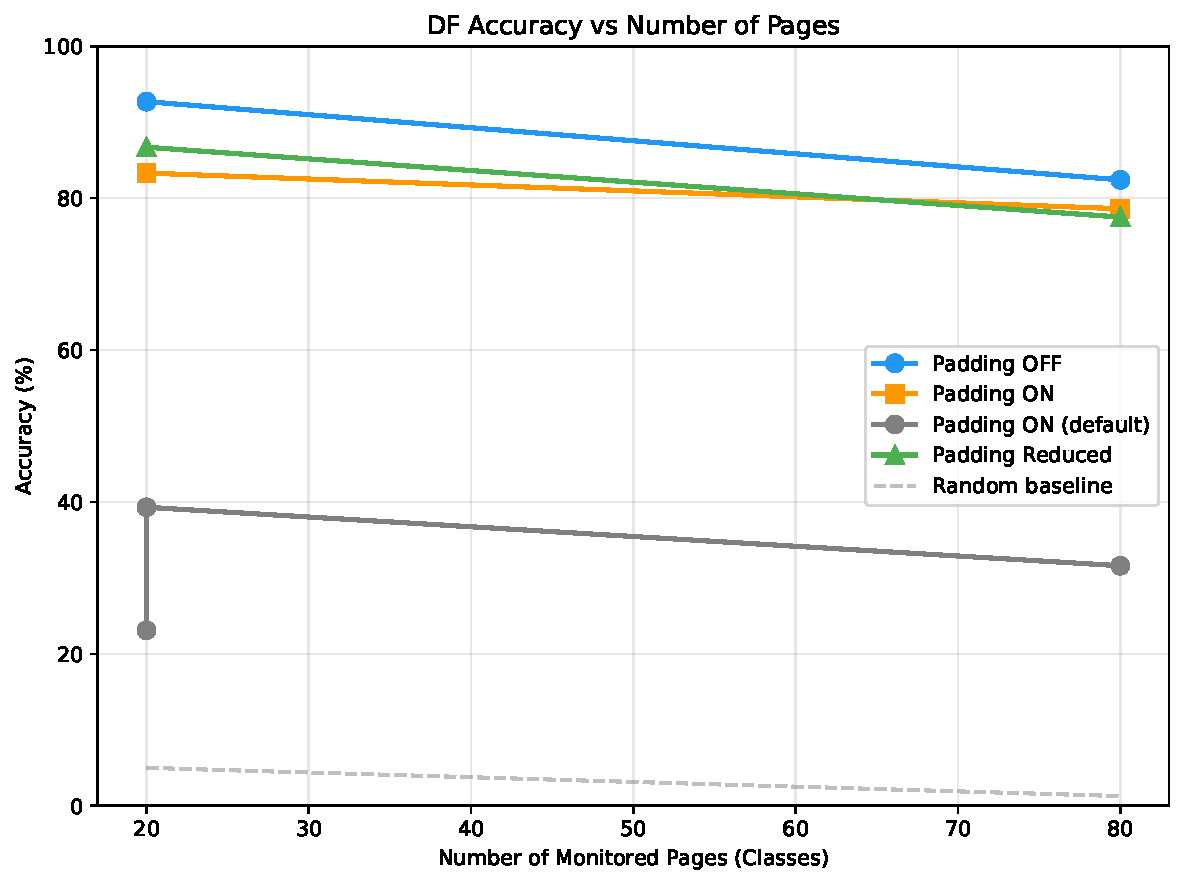
\includegraphics[width=0.85\textwidth]{../../images/results/accuracy_vs_pages.pdf}
    \caption{Accuracy als Funktion der Klassenanzahl, getrennt nach Padding-Modus. Eigene Darstellung.}
    \label{fig:eval_acc_vs_pages}
\end{figure}

\subsection{Effekt von Circuit Padding}
\label{sec:eval_padding_effekt}



\begin{figure}[H]
    \centering
    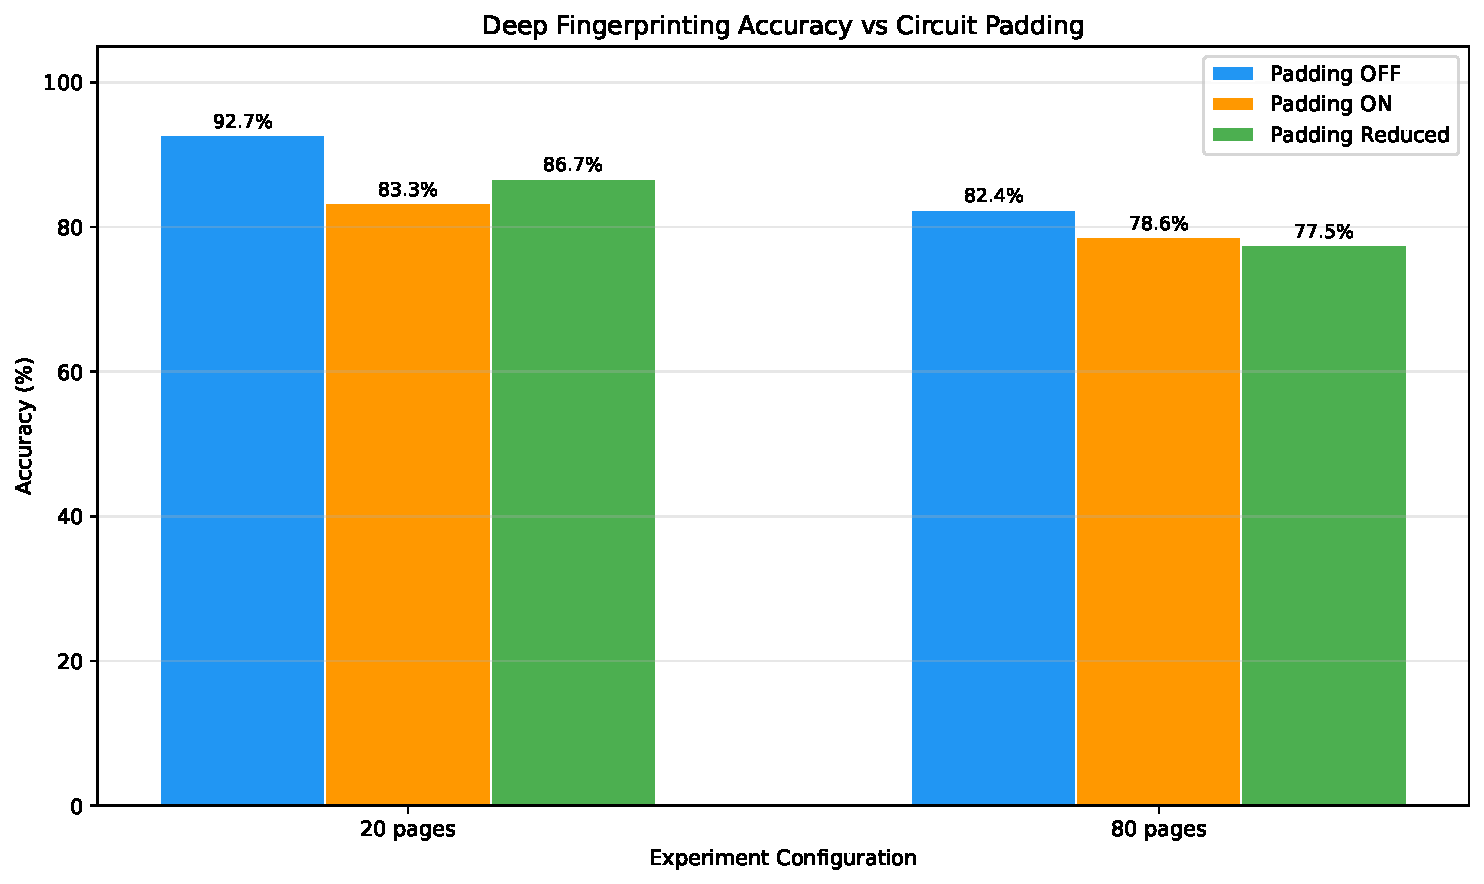
\includegraphics[width=0.85\textwidth]{../../images/results/padding_comparison.pdf}
    \caption{Accuracy-Vergleich der drei Padding-Modi für 20 und 80 Klassen. Eigene Darstellung.}
    \label{fig:eval_padding_comp}
\end{figure}

\begin{figure}[H]
    \centering
    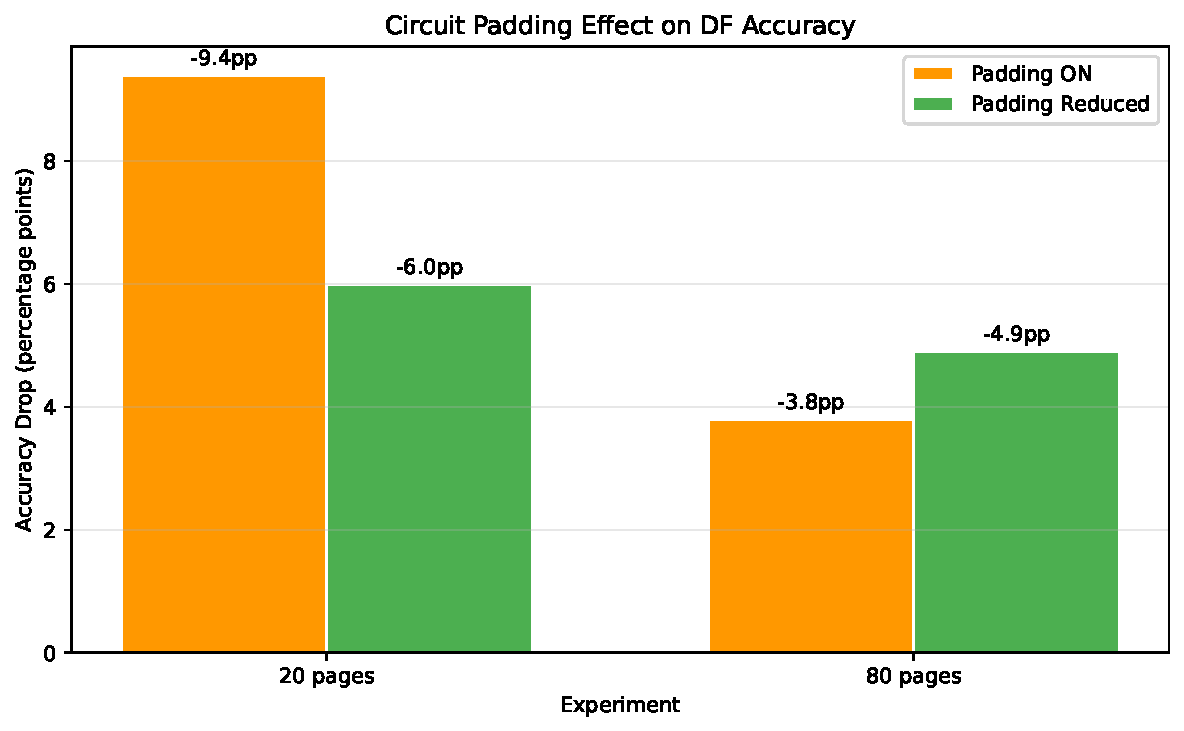
\includegraphics[width=0.75\textwidth]{../../images/results/padding_delta.pdf}
    \caption{Veränderung der Accuracy gegenüber der Baseline (OFF) in Prozentpunkten. Eigene Darstellung.}
    \label{fig:eval_padding_delta}
\end{figure}

\subsection{Reduced Padding}
\label{sec:eval_reduced}



\begin{figure}[H]
    \centering
    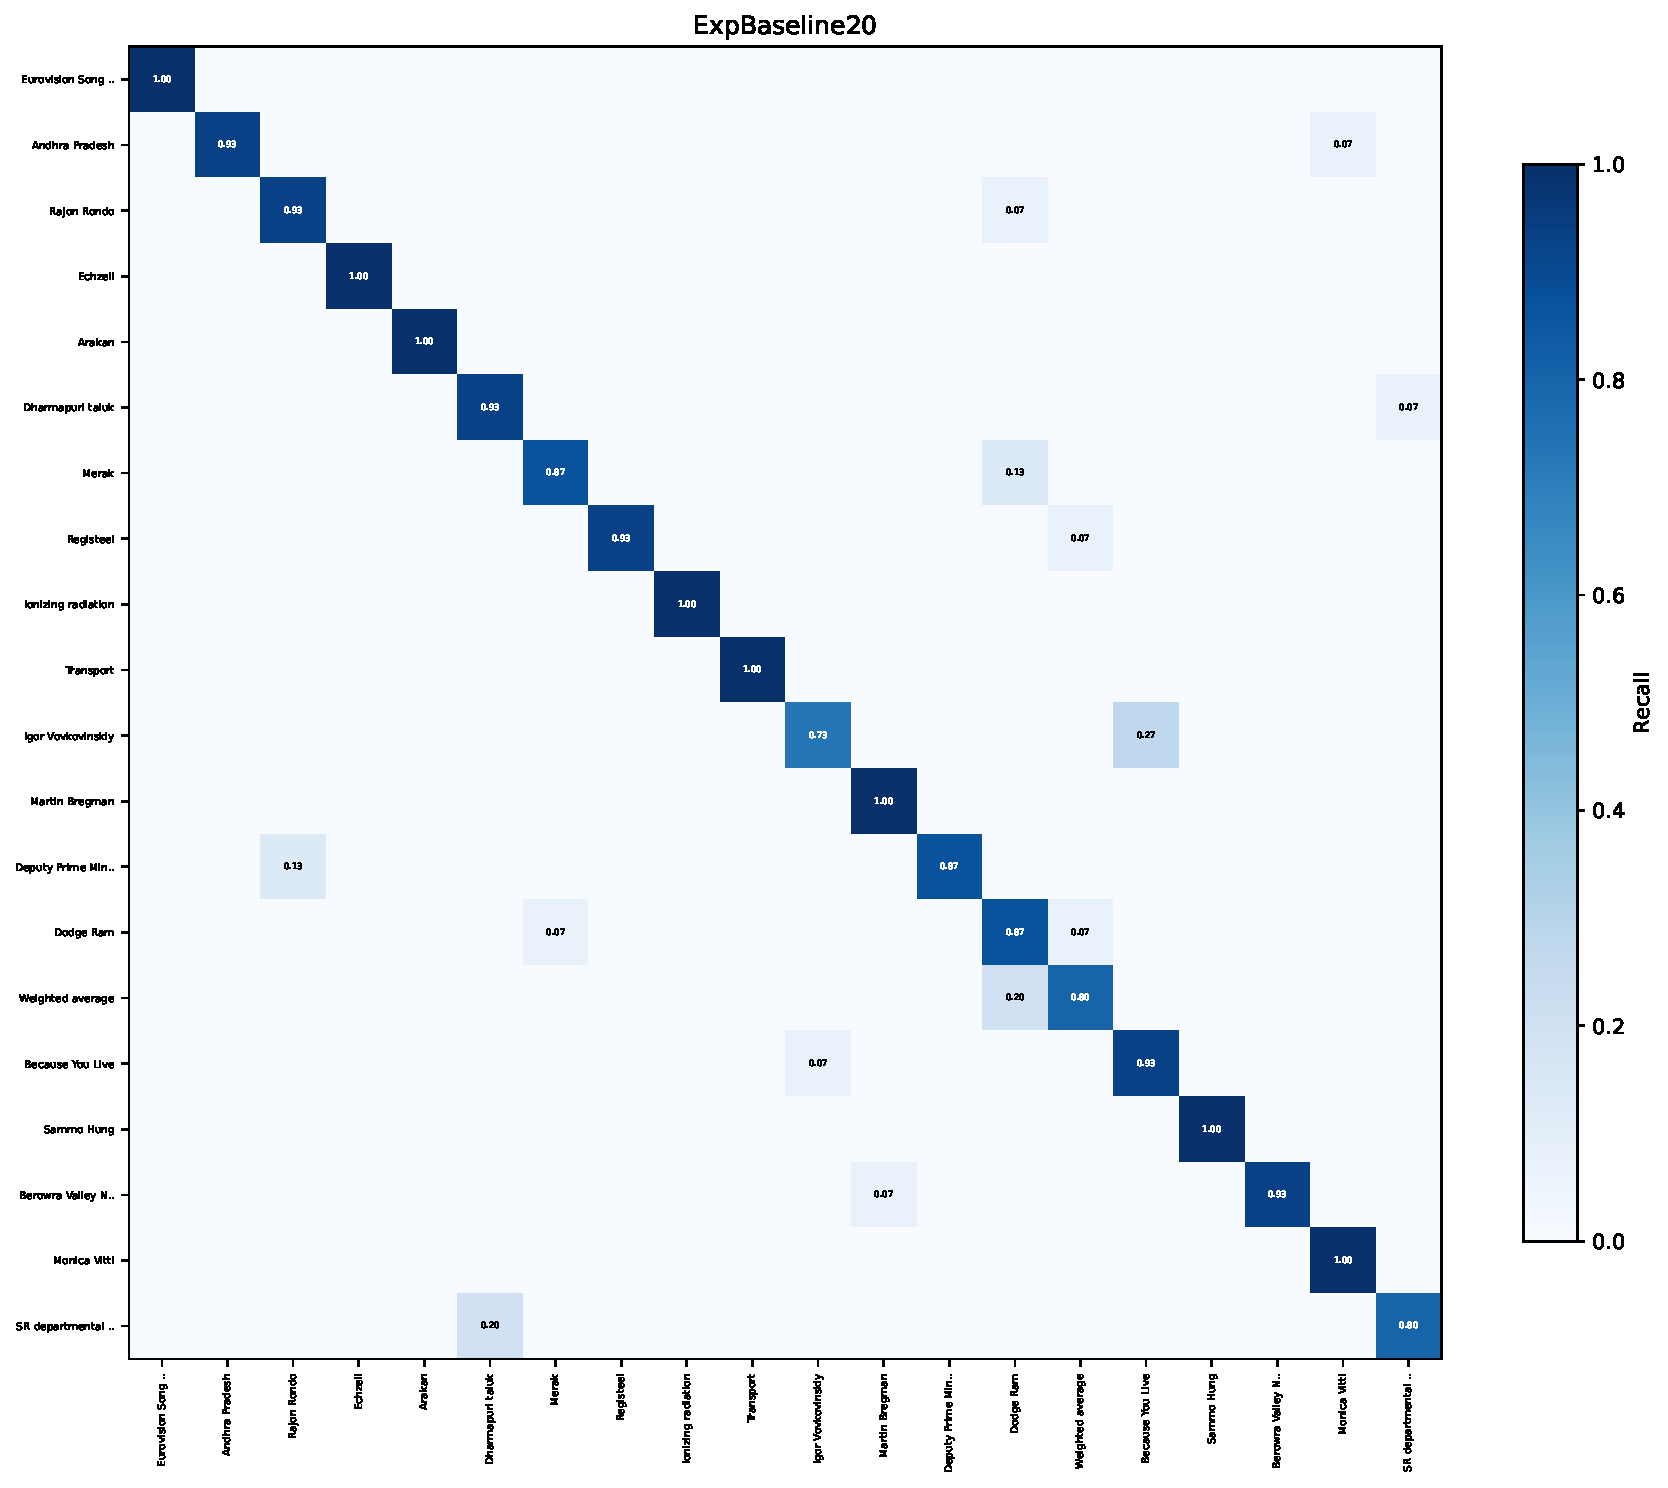
\includegraphics[width=0.55\textwidth]{../../confusion_baseline20.pdf}
    \caption{Konfusionsmatrix der Baseline mit 20 Klassen. Eigene Darstellung.}
    \label{fig:eval_confusion_baseline20}
\end{figure}

\begin{figure}[H]
    \centering
    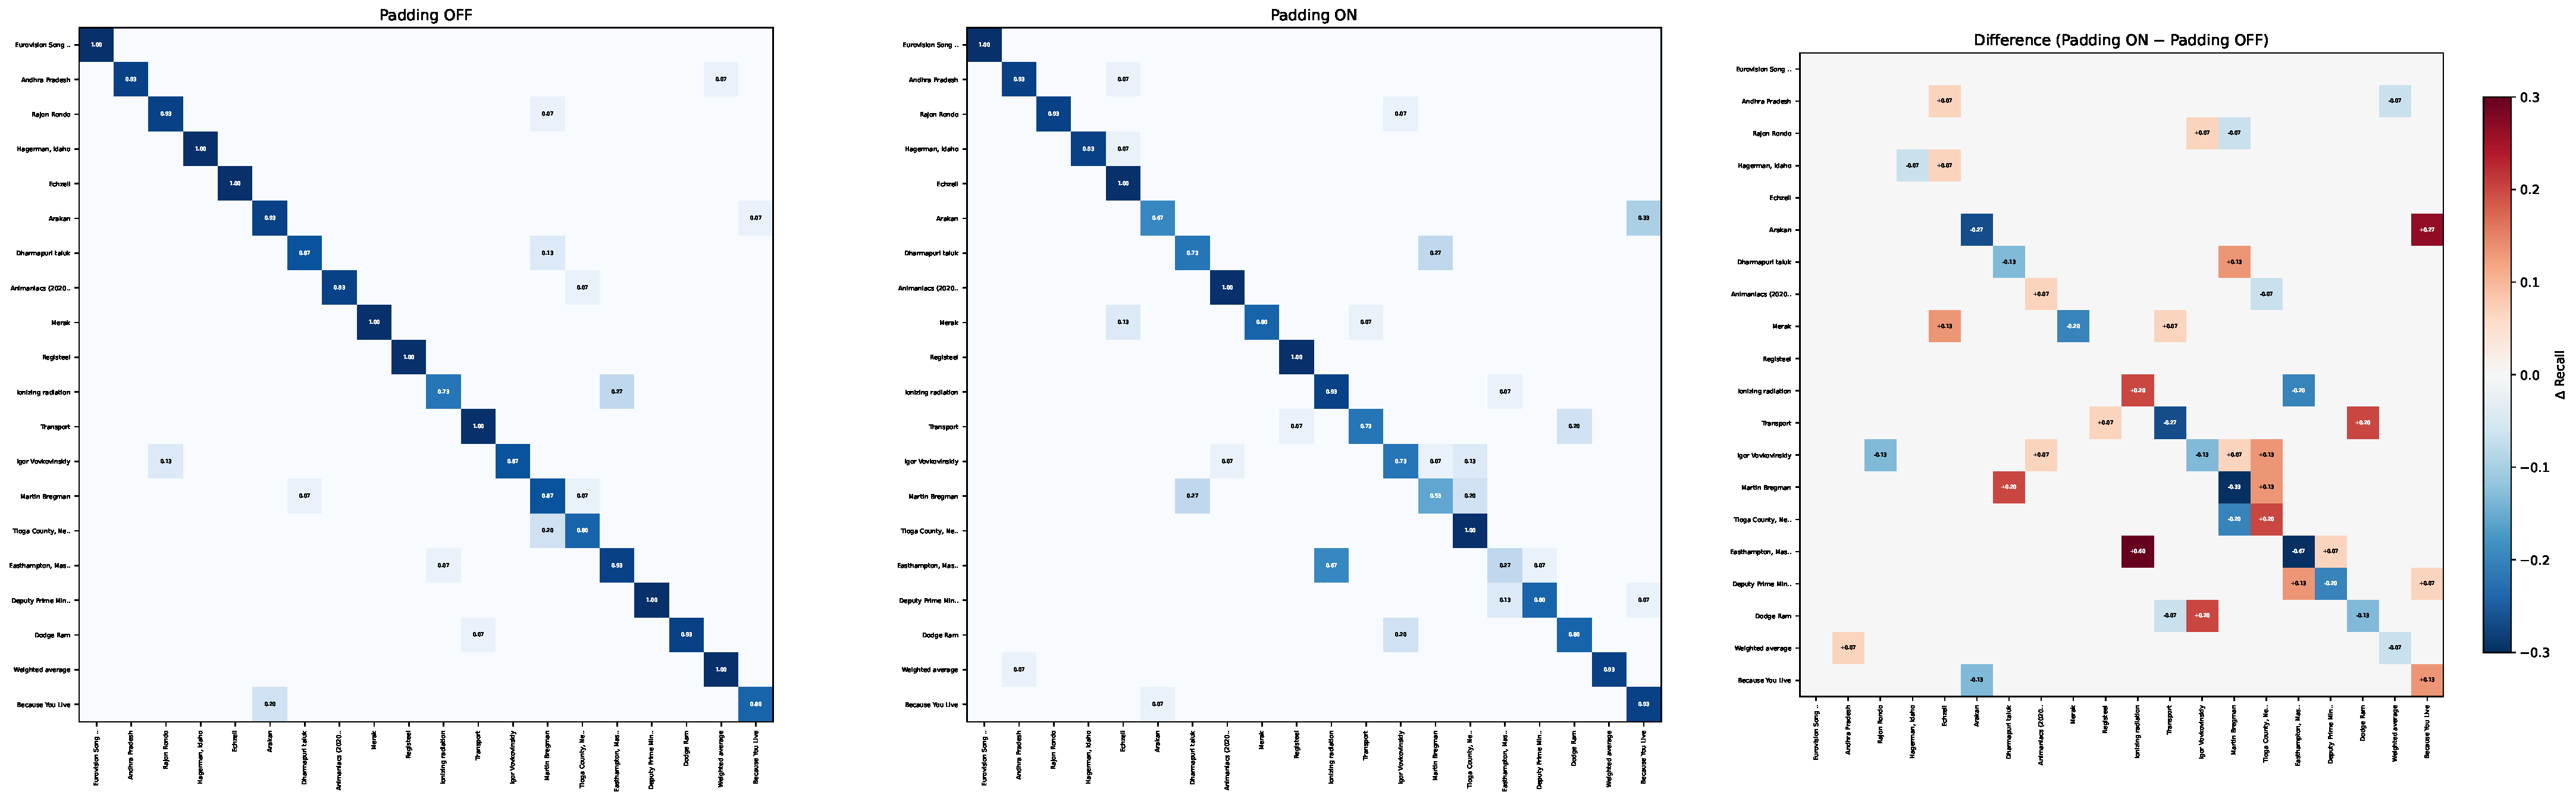
\includegraphics[width=\textwidth]{../../confusion_comparison_20.pdf}
    \caption{Konfusionsmatrizen OFF (links) und ON (rechts) bei 20 Klassen. Eigene Darstellung.}
    \label{fig:eval_confusion_comparison20}
\end{figure}

\begin{figure}[H]
    \centering
    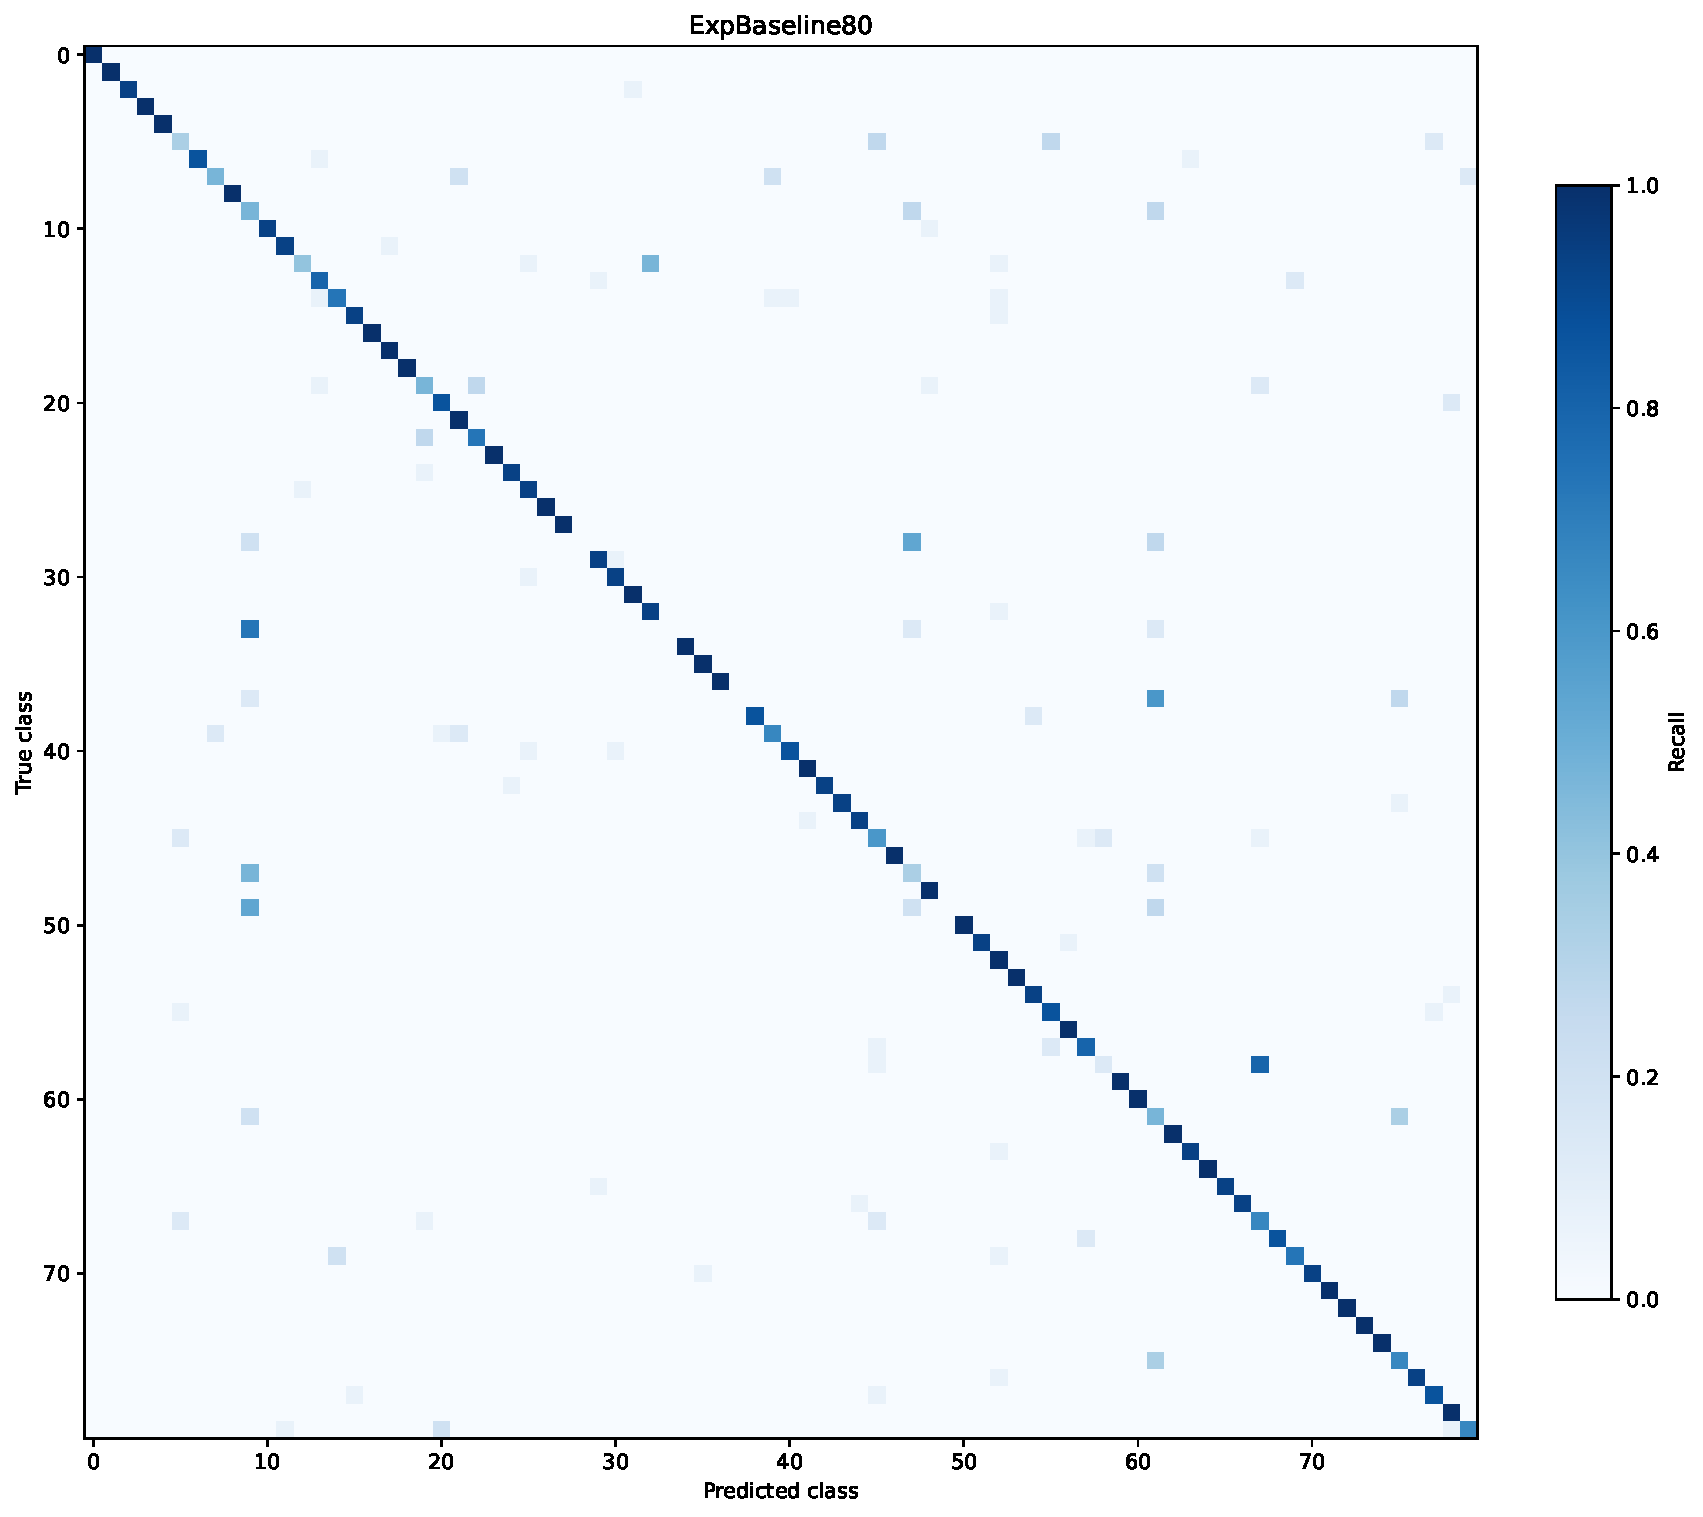
\includegraphics[width=0.55\textwidth]{../../confusion_baseline80.pdf}
    \caption{Konfusionsmatrix der Baseline mit 80 Klassen. Eigene Darstellung.}
    \label{fig:eval_confusion_baseline80}
\end{figure}



\todo{TODO}

\begin{figure}[H]
    \centering
    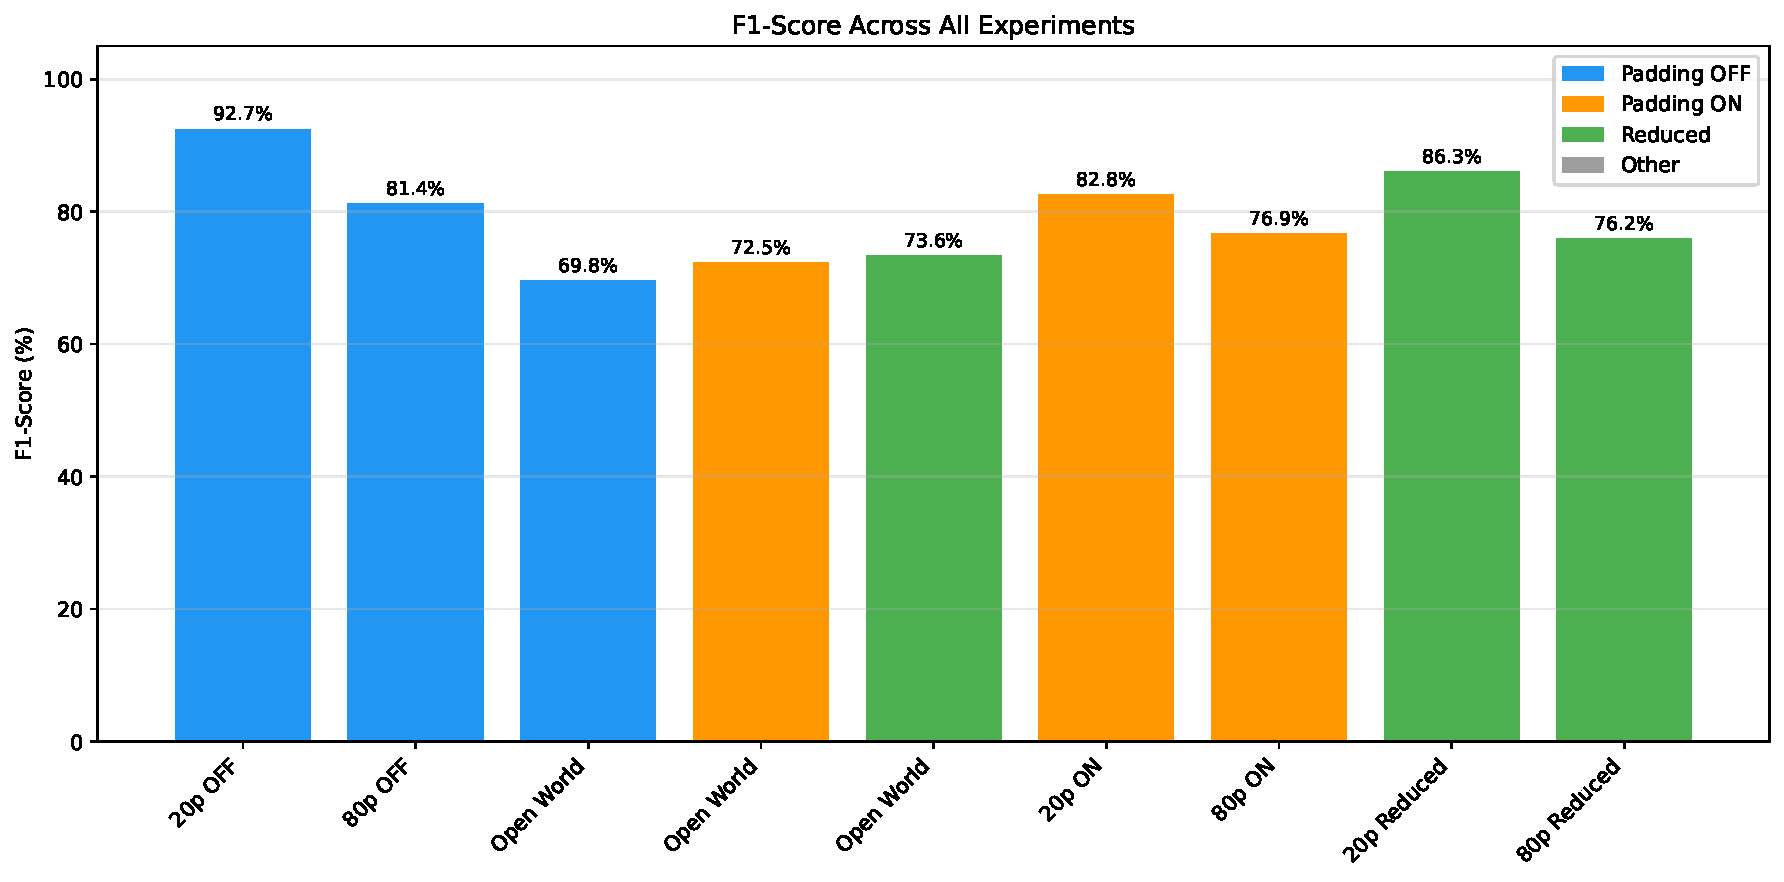
\includegraphics[width=0.85\textwidth]{../../images/results/f1_comparison.pdf}
    \caption{F1-Wert über alle Hauptexperimente. Eigene Darstellung.}
    \label{fig:eval_f1}
\end{figure}


\begin{table}[H]
    \centering
    \caption{Open-World-Resultate für 80 überwachte Seiten in einem Topf von 280 Quellseiten. Quelle: \texttt{ExperimentLogs.csv}.}
    \label{tab:eval_openworld}
    \begin{tabular}{lrrrr}
        \hline
        Padding & Accuracy & Precision & Recall & F1-Wert \\
        \hline
        OFF & 68.3\,\% & 67.9\,\% & 74.6\,\% & 69.8\,\% \\
        ON  & 70.7\,\% & 72.5\,\% & 75.6\,\% & 72.5\,\% \\
        \hline
    \end{tabular}
\end{table}


\section{Ressourcen und Performance}
\label{sec:eval_performance}

Ergänzend zu den klassifikationsbezogenen Resultaten wird der Ressourcenverbrauch des Simulationsservers \texttt{shadowsrv-001} während der Experimente protokolliert.
Dazu wird das Skript \texttt{perfmon.py} verwendet, das in einem Intervall von fünf Sekunden Werte aus \texttt{/proc/stat}, \texttt{/proc/meminfo}, \texttt{statvfs} und \texttt{/proc/loadavg} ausliest und in eine tagesweise rotierte \texttt{CSV}-Datei schreibt.
Der hier dargestellte Ausschnitt umfasst rund 70 Minuten und 853 Messpunkte aus dem laufenden Experiment \texttt{exp-tamaraw-80}.

\begin{figure}[H]
    \centering
    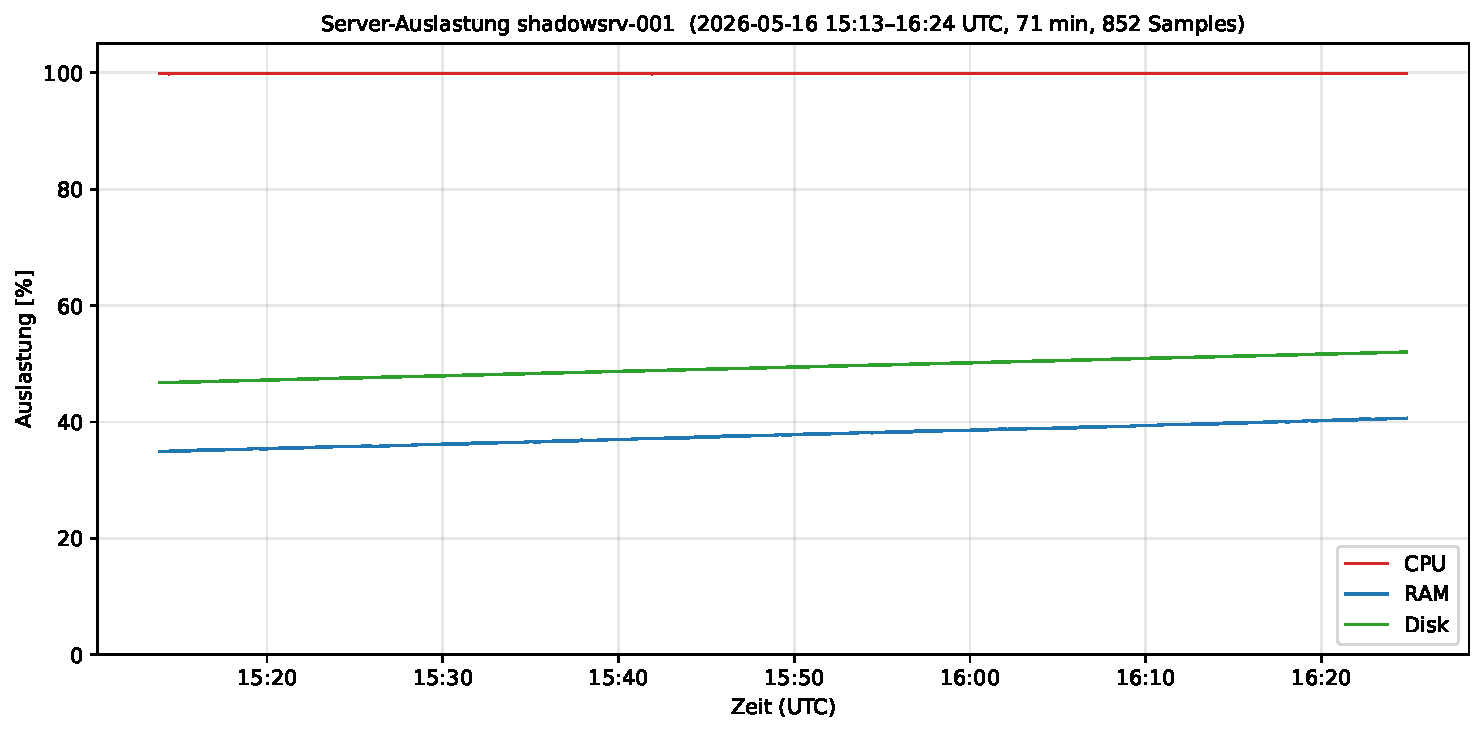
\includegraphics[width=0.95\textwidth]{../../images/results/perfmon.pdf}
    \caption{Auslastung von CPU, Arbeitsspeicher und Disk auf \texttt{shadowsrv-001} während \texttt{exp-tamaraw-80}. Quelle: \texttt{perfmon-logs/perfmon-2026-05-16.csv}.}
    \label{fig:eval_perfmon}
\end{figure}

Die CPU-Auslastung liegt durchgehend bei rund 99.9\,\%, was angesichts von 32 Kernen und einem 1-Minuten-Load-Average von 35.8 (Maximum 38.6) eine leicht überzeichnete Ausnutzung der verfügbaren Rechenkapazität bedeutet.
Der Arbeitsspeicher steigt im Beobachtungsfenster von 44 GB auf 51 GB an und bleibt damit bei rund 40\,\% der verfügbaren 126 GB.
Die Disk-Auslastung wächst im selben Zeitraum von 73 GB auf 81 GB und liegt bei rund 52\,\% der 156 GB grossen Partition.

Aus diesen Werten lässt sich ableiten, dass die CPU der limitierende Faktor der gewählten Netzwerkgrösse ist, während Arbeitsspeicher und Disk im untersuchten Szenario Reserven bieten.
Eine ausführlichere Auswertung über mehrere Experimente hinweg, inklusive Aufschlüsselung nach Simulationsphasen wie tornettools-Generierung, Shadow-Lauf und Auswertung, folgt nach Abschluss von \texttt{exp-tamaraw-80}.

\todo{Performance-Werte für die übrigen Experimente nachtragen und Diskussion auf Engpässe (CPU, Disk-IO) erweitern.}

\section{Bandbreiten-Overhead}
\label{sec:eval_bandwidth}

\todo{Tamaraw-Bandbreiten-Overhead mit \texttt{pcap\_overhead.py} aus \texttt{exp-tamaraw-20} gegen \texttt{exp-baseline-20} berechnen.
Mittelwert und Median der Up-, Down- und Gesamtbytes pro Visit angeben, dazu den Paket-Overhead.
Resultate als kurze Tabelle, optional zusätzlich Boxplot der Per-Visit-Bytes aus dem CSV-Export.}